\chapter{Introduction}
\label{chap:introduction}

Financial institutions make decisions to buy or sell assets for many reasons, including: customer requests, fundamental analysis\cite{fundamental-analysis}, technical analysis\cite{technical-analysis}, top-down investing\cite{td-investing}, and bottom-up investing\cite{bu-investing}.
High-level trading strategies oftentimes define how an institution positions itself in financial markets and, if applicable, towards its customers.
Regardless of the high-level trading strategy that is applied, the invariable outcome is a decision to buy or sell assets.
This work aims to take a step towards answering the important question of how one can optimize a purchase or sale of an asset on a stock exchange with the use of reinforcement learning techniques.
The subsequent sections will elaborate this problem briefly and state the research objectives of this work.
We will list the contributions made to research communities throughout this work, followed by a brief overview of the structure of this report.

\section{Context and Problem Statement}
\label{sec:problem-statement}

We are concerned about the way assets, specifically \textit{securities} (exchange traded assets), are traded on stock exchanges.
There is little consensus as to when corporate stock was first traded; some argue that the exchange, in the form we know it today, dates back as far as 1531, when East Indian Company stock was traded in Antwerp\cite{stock-exchange}.
Modern financial markets such as the London Stock exchange (LSE), the New York Stock Exchange (NYSE), but also the numerous crypto-currency exchanges which have appeared suddenly in the last few years, all rely on the very same principles as back then.
They allow participants (called "traders") to buy or sell a given amount of a security at a particular price.
In the late 1990s, the regulatory authorities started to let traders access the markets using electronic communications networks (ECNs) and so a new era dawned \cite{patterson2012dark}.
Since then, high frequency trading (HFT) and sophisticated algorithmic trading vehicles have made up a substantial and ever-increasing part of electronic market participants.
Their servers are oftentimes located within exchanges and specialized computer networks have been constructed to provide millisecond-level advantage in the arbitrage of trades between exchanges.
Ever since, traders without such equipment and techniques have felt that they are at a disadvantage in such an environment \cite{patterson2012dark}.
While anything except trading through electronic channels would be unthinkable today, a certain gap still exists between trading companies that have fibre access to the exchanges or supporting algorithms and investors who do not.
As a result, investors are forced to take an initial loss into account when buying or selling securities, which they might not even be aware of.
In order to understand why these losses are incurred, we have to have a basic understanding of a so-called order book and how securities are bought at an exchange.

\begin{figure}[H]
    \centering
    \makebox[\linewidth]{
        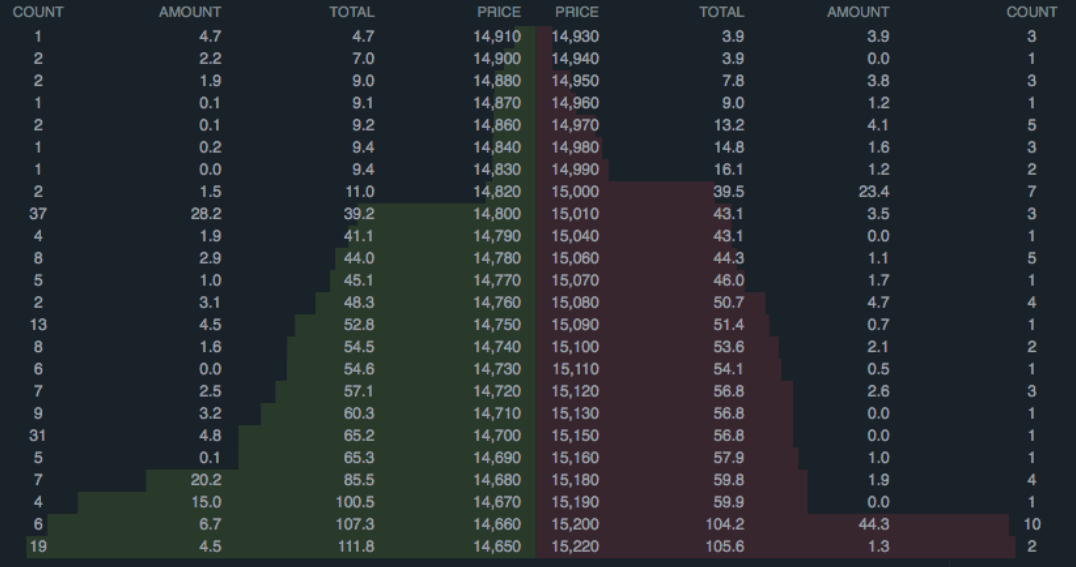
\includegraphics[width=12cm]{orderbook-gdax.png}
    }
    \caption{Order book snapshot: https://www.bitfinex.com/t/BTC:USD}
    \label{fig:intro-orderbook}
\end{figure}

Figure \ref{fig:intro-orderbook} shows a snapshot taken at some time $t$ of the trading pair Bitcoin (BTC) versus US dollar (USD) taken on the Bitfinex\footnote{https://www.bitfinex.com} cryptocurrency exchange.
The order book shows two columns, the parties who are willing to buy are on the left and the parties who are willing to sell are on the right.
The two columns indicate the number of buyers and sellers (\textit{count}) who are willing respectively to buy and sell a certain \textit{amount} for a given \textit{price}.
The column \textit{total} is the cumulative sum of the amount, or volume, on each side.
The difference between the figures in each column is the \textit{spread}.
In this particular case, the current best \textit{bid} price--at which someone is willing to buy--is \$14,910.00 and the best ask-price at which someone is willing to sell, is \$14,930.00.
Therefore, the spread is currently \$20.00.
\\
\\
Suppose we want to buy 1.0 BTC.
Two possible ways to do so are:
\begin{enumerate}
    \item Buy 1.0 shares immediately for \$14,930.00 from a seller. To do so, we submit a \textit{market} order.
    \item State a price at which we are willing to buy 1.0 shares at price $p$, for example at \$14,910.00, and wait until someone is willing to sell at this price. To do so, we submit a \textit{limit} order.
\end{enumerate}

Both types of orders come with their advantages and disadvantages.
A market order ensures that we will be able to acquire the stated amount of shares immediately for \$14'930.00, provided that no one else  has a prior claim to them and that the seller does not cancel his/her listing.
In this case, we are automatically willing to pay the next available best price.
However, we do pay a premium compared to the limit order since ask prices are listed higher than bid prices and the more shares one wants to buy, the more sellers we have to contact and accept their offers at an increased price.
With a limit order, the exchange guarantees that we will pay \$14,910.00 or less.
That is, when a seller is willing to sell for the stated price or less, the exchange will match the offers of both parties.
However, this comes with the risk that we will never be able to buy if nobody is going to sell at the demanded price, and this will force us to buy the shares demanded at a later point in time.
As the price of a share evolves over time, we might get lucky and be able to buy at a cheaper price than at the time of the initial attempt.
The other scenario is that the price did not develop in our favour such that we have to buy at a higher price later on; thus, we pay a so-called \textit{opportunity cost}.
A third order type, the \textit{cancel} order, allows a trader to cancel his/her previously posted limit or market order at any given point in time.
%Ultimately, we have a brief understanding of what traders are allowed to do at a stock exchange.
%We will now elaborate briefly how such a relatively simple concept of an order book and three types of orders can lead to a diverse range of situations a trader can find himself whereas at times this may be beneficial for his intentions and at times it will lead to paying a premium.
%If a seller realizes that we are about to buy for price $p$ at which is was willing to sell, he then could \textit{cancel} his offer as his incentive is to sell for a higher price.
%Perhaps this has been his/her intention to only post an offer but withdrawal as soon as a counter-offer will be listed that is close to his/her price.
%This method is known as \textit{quote stuffing}.

With this brief understanding of how traders can interact with the exchange, we can define the problem of \textit{order placement} as follows.
Order placement determines the price at which a trader places its order.
The aim of optimizing order placement are to minimize the opportunity cost and, ideally, achieve a more favorable price payable (or receive) than what is currently being offered at the market price.
Literature therefore specifies a time scale of from ten to one hundred seconds within which a trader has to complete his task of either buying or selling the shares \cite{guo2013optimal}.
A time scale of less than ten seconds applies in high frequency trading and one of above 100 seconds is known as \textit{order execution optimization}.
Thus, could we define order placement optimization as the price $p$ at which one should attempt to buy or sell $i$ shares within a time horizon $H$ of 100 seconds?
As we shall see, optimizing placement is not as trivial as one might think, even though the concepts of the order book and the three order types a trader can choose from are admittedly simple.
There are various properties in a limit order book, as well as the behaviour of the market participants, that changes over time.
All of which can drastically interfere with the intention of buying and selling.
Furthermore, since the foundation of electronic trading networks and algorithmic trading, the amount and sophistication of other market participants has been ever-increasing, with everyone aiming for an advantage over others.
%However, the prices for some financial products, including crypto-currencies, are very volatile such that it is likely to be able to buy for less than what is offered at the mentioned time $t$.
%In addition, there might be buyers and sellers in the near future which would consume our order.
%Thus, placing orders \textit{deeper} in the book and wait could be beneficial.
%
%According to Guo et. al. \cite{guo2013optimal} algorithmic trading is based on two different time scales: \textit{order execution} concerns about optimally slicing big orders into smaller ones in order to minimize the \textit{price impact}, that is, on a daily or weekly basis.
%\textit{Order placement} on the other hand concerns about optimally placing orders within ten to hundred seconds.
%In this thesis we are concerned about the latter, which conforms the context of the problem:

The fact that reinforcement learning functions by maximizing rewards makes this technique unarguably suitable in this context.
That is, how to place orders according to the given market condition and therefore protect an investor form paying the aforementioned premium to other participants in the market.
Ideally, such a learner will be able to foresee short-term trend changes such that the investor ultimately benefits from a better price at which to buy or sell the asset. 

\section{Research objectives}
\label{sec:intro-rq}

This work extends the findings of Kearns et. al. who have studied the behavior of order placement and order execution\cite{nevmyvaka2005electronic}, and developed a reinforcement learning strategy\cite{nevmyvaka2006reinforcement} for the purposes of optimization.
Their work explains how features derived from order book data were pre-processed and applied to a reinforcement learning algorithm which is similar to Q-Learning.
In this thesis, rather than constructing features by hand, we will describe a particular instance of how deep reinforcement learning techniques were employed in order to benefit from patterns in raw market data.
In addition, the cryptocurrency domain was chosen, instead of the traditional stock market.
Furthermore, while the previously mentioned work of Kearns et al. had success in using pre-processed market data as features, we believe that raw market data in combination with deep reinforcement learning can be equally successful.
Hence, our ambition is to determine if deep reinforcement learning is perhaps an even more suitable choice in order to deal with unexpected market situations.
Therefore we have formulated the following research question to be answered in this thesis:
\\
\\
\textbf{RQ 1:} How can the application of deep reinforcement learning contribute to the optimization of limit order placement?
%\textbf{RQ 1 (B):} Which cryptocurrency market events enable us to foresee opportunities to place limit orders at a favorable price with the use of deep reinforcement learning?
\\
\\
\textit{We chose to divide the research question into sub-questions as this choice follows the logical structure of this document and provides an understanding of the steps taken in order to give an answer to the main research question.}

\begin{quote}
\begin{description}
    \item[RQ 1.1:] Which historical market data patterns drive market participants to buy or sell assets, and how can these patterns be incorporated into features used by a deep reinforcement learning agent?
\end{description}
    Traders participating in financial markets, including cryptocurrency markets, can submit and cancel orders to trade shares.
    These events are recorded by the cryptocurrency exchange and are publicly accessible as raw market data.
    We intend to find patterns in the data which reflect the behavior of these market participants.
    The patterns found will form the basis of hypotheses suggesting that some behavioral patterns are more likely to lead traders either to buy or sell an asset in the short term.
    Whenever a hypothesis is true, one can determine a favorable price at which to buy or sell the asset, and hence, mitigate the impact of the order placement problem.
    Thus, we have to determine how to and construct features with the patterns found incorporated that enable deep reinforcement learning agents to learn an order placement strategy.

\begin{description}
    \item[RQ 1.2:] How can one design a reinforcement learning environment and agents, in the context of order placement?
\end{description}
    In order to simulate and understand the outcome of order placement and, more importantly, build a reinforcement learning environment that allows interaction with agents, this work will suggest a way of translating the given problem into a reinforcement learning context.
    Consequently, we are required to build a framework which should provide collection and market data processing capabilities in order to reproduce a historical order book that serves as a data source.
    Further, we require that the framework provide the functionality of a match engine which emulates the functionality of a stock exchange that can match orders and determine the resulting price paid (or received) according to a historical order book.
    Ultimately, a reinforcement learning environment should be built to simulate and evaluate order placement.
    The environment should allow direct user interaction in order to place orders on demand and allow interaction with agents which act as intelligent traders.
    Therefore, we have made use of the OpenAI Gym\footnote{https://github.com/openai/gym} library and we contribute our work to the community to enable further investigations to be carried out.
    
    Further, we shall then build two reinforcement learners which will both act as intelligent traders and thereby place limit orders that provide an incentive to buy or sell an asset at a favorable price.
    Both agents should be driven by an end-to-end learning process by which the agent improves based on the outcome of the orders placed and ultimately learns a strategy for  buying and selling shares at favorable prices.
    The former agent is an adaptation of the well- known Q-Learning algorithm and optimizes only in accordance with the amount of assets to buy or sell and the given time horizon.
    This agent is a deep reinforcement learning agent that makes use of a convolutional neural network in order to detect patterns in market data.

\begin{description}
    \item[RQ 1.3:] How can one evaluate a reinforcement learning environment and agent in the context of order placement?
\end{description}
    The ability to quantify the capabilities of a limit order placement strategy learned by a reinforcement learning agent is of significant importance when answering the main research question in this thesis.
    Since there is no literature available which states results for the exact same data set, nor for any data set within the crypto- currency domain, a procedure has to be introduced by which different learning approaches and features considered can be evaluated.
    Therefore a measure is to be taken that is well-suited to the determination and comparison of the capabilities of a reinforcement learning agent in the order placement context.
    Furthermore, the evaluation procedure should identify the extent to which a limit order placement can be optimized in a given historical data set.
    As a result, the evaluation shall serve as a reliable measure of how well a learned order placement strategy performs.
    
\begin{description}
    \item[RQ 1.4:] In which way do the constructed features enable a reinforcement learning agent to improve the way it places orders?
\end{description}

    The significance of deep reinforcement learning and the use of features derived from market data has to be determined in the application of order placement.
    The findings shall be compared to the performance achieved by a learner which has less information available, as well as the previously identified limitations of the market data available.
    Finally, the limitations of a learned strategy are to be identified.
\end{quote}

\section{Document structure}

In Chapter \ref{chap:preliminaries}, we first provide background information to the reader on the components of a stock exchange. %and the fundamentals of the closely related time series.
Further, we make the reader familiar with (Deep) Reinforcement Learning.
In Chapter \ref{chap:related-work}, we elaborate on the behavior of order placement followed by approaches of both statistical and machine learning nature.
Chapter \ref{chap:data} explains the process of data collection and preparation which was carried out prior to its use in the subsequent chapters.
Chapter \ref{chap:setup} explains the experimental setup of the reinforcement learning environment, the agents and the way processed features are used.
In Chapter \ref{chap:analysis}, we analyze the data, carry out order placement, and include reasons for our findings.
Finally, in Chapter \ref{chap:discussion}, we formulate a conclusion of our findings and state a future research direction.
